%\documentclass{article}
\documentclass{www2010-submission}
\usepackage{times}
%\usepackage{uist}
\usepackage{url}
\usepackage{graphics}
\usepackage{color}
%
%\newcommand{\want}[1]{{[\color{blue} WANT: #1]}}
%\newcommand{\todo}[1]{{[\color{blue} TODO: #1]}}
%\newcommand{\idea}[1]{{[\color{blue} IDEA: #1]}}
%\newcommand{\node}[1]{{[\color{blue} NOTE: #1]}}

\newcommand{\want}[1]{}
\newcommand{\todo}[1]{}
\newcommand{\idea}[1]{}
\newcommand{\node}[1]{}


\begin{document}

\toappear

\bibliographystyle{plain}

\title{Highlighting Disputed Claims on the Web}

%%
%% Note on formatting authors at different institutions, as shown below:
%% Change width arg (currently 7cm) to parbox commands as needed to
%% accommodate widest lines, taking care not to overflow the 17.8cm line width.
%% Add or delete parboxes for additional authors at different institutions. 
%% If additional authors won't fit in one row, you can add a "\\"  at the
%% end of a parbox's closing "}" to have the next parbox start a new row.
%% Be sure NOT to put any blank lines between parbox commands!
%%

\numberofauthors{5}

\author{
	Author list to be determined
}

\author{
\alignauthor Rob Ennals\\
       \affaddr{Intel Labs Berkeley}\\
       \affaddr{2150 Shattuck Ave}\\
       \affaddr{Berkeley, CA, USA}\\
       \email{robert.ennals@intel.com}
\alignauthor Beth Trushkowsky\\
       \affaddr{Computer Science Division}\\
       \affaddr{University of California at Berkeley}\\
       \affaddr{Berkeley, CA, USA}\\
       \email{trush@cs.berkeley.edu}
\alignauthor John Mark Agosta\\
       \affaddr{Intel Labs Santa Clara}\\
       \affaddr{2200 Mission College Blvd}\\
       \affaddr{Santa Clara, CA, USA}\\
       \email{john.m.agosta@intel.com}
}

%\sloppy

\additionalauthors{Tye Rattenbury and Tad Hirsch, Intel Research Principles and Practices,\texttt{[tye.rattenbury,tad.hirsch]@intel.com}}


\maketitle

%RULE: Don't cite media reports unless I have to - some reviewers don't like it


\abstract

We describe Dispute Finder, a browser extension that alerts a user when information they read online is disputed by a source that they might trust. Dispute Finder examines the text on the page that the user is browsing and highlights any phrases that resemble known disputed claims. If a user clicks on a highlighted phrase then Dispute Finder shows them a list of articles that support other points of view.

Dispute Finder builds a database of known disputed claims by crawling web sites that already maintain lists of disputed claims, and by allowing users to enter claims that they believe are disputed. Dispute Finder identifies snippets that make known disputed claims by running a simple textual entailment algorithm inside the browser extension, referring to a cached local copy of the claim database.

In this paper, we explain the design of Dispute Finder, and the trade-offs between the various design decisions that we explored. 

\category{H.4.m}{Information Systems}{Miscellaneous}
\category{H.4.2}{Information Systems}{Decision Support}
\category{H.5.2}{User Interfaces}{Graphical User Interfaces}

\terms{Design, Human Factors}

\keywords{Sensemaking, Annotation, Argumentation, Web, CSCW}


\tolerance=400 
  % makes some lines with lots of white space, but 	
  % tends to prevent words from sticking out in the margin

\section{Introduction}

\todo{update screenshots}
\todo{should this be spun as about news, or information in general}
\todo{need to talk more about what we know about people}
 
% The last few years have seen the rapid decline of printed newspapers and rapid rise of the web as a source of news~\cite{pew-news?}.

The web contains a huge amount of information, but some of this information is factually incorrect and some sites present only one side of a contentious issue~\cite{Herman2002}. If a user is to gain a broad understanding of a topic then they will need to either spend time searching for alternative points of view, or restrict themselves to sources that they believe they can trust to provide accurate and balanced information. Even when a user spends time investigating every claim that they think might be disputed, they can still be misled by information that they had not realized was disputed.

In recent years, we have seen the emergence of a new class of tools that help users recognize and make sense of disputed information on the web. In this paper, we describe Dispute Finder, a tool that alerts a user when a web page they are reading appears to be making a claim that is disputed by a source that they might trust.

\begin{figure}[tb]
	\begin{center}
	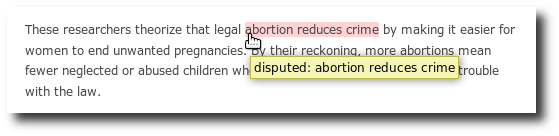
\includegraphics[width=8.5cm]{pictures/highlight_abortion.png}
	\caption{Dispute Finder highlights text snippets that make disputed claims.}
	\label{highlight}
	\end{center}
\end{figure}

\begin{figure}[tb]
	\begin{center}
	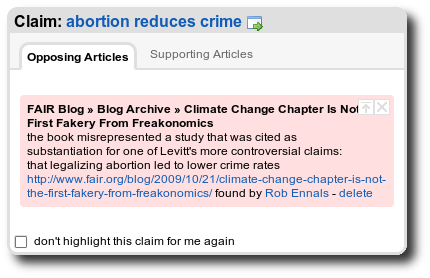
\includegraphics[width=7cm]{pictures/popup_abortion_shadow.png}
	\caption{Click on a highlighted snippet to see a popup interface with articles arguing for and against the claim.}
	\label{claimview}
	\end{center}
\end{figure}
\todo{Popup interface should contain a ``don't mark this'' button}

\todo{More screenshots/graphs/visual information}

\todo{word this better}\todo{update all screenshots}

%In this paper we describe Dispute Finder, a tool that alerts a user when information they read online is disputed by a source that they might trust. Our hope is that Dispute Finder will make it easier for a user to gain a broad view of a topic that they are interested in by exposing them to different points of view.

A user can install Dispute Finder as an extension to the Firefox\footnote{http://www.mozilla.org/firefox} web browser. When installed Dispute Finder will highlight snippets of text that make disputed claims (Figure~\ref{highlight}). 
If a user clicks on a highlighted snippet, Dispute Finder will show articles that put forward alternative points of view,  each of which is from a source we believe the user might trust (Figure~\ref{claimview}). 

Dispute Finder consists of a server-side database and a Firefox browser extension. The database contains a set of known disputed claims that frequently appear on the web. A disputed claim is a statement about the world that some people disagree with. For example ``global warming is a hoax'', ``gun control will reduce crime'', ``Eskimos have many words for snow'', or ``margarine is healthier than butter''. A claim can be stated in many ways. For example ``margarine is healthier than butter'' and ``butter is worse for you than margarine'' are {\it paraphrases} of the same claim. For each claim, the database contains links to articles on the web that support or oppose it, and hints about how to recognize that disputed claim on the web (Figure~\ref{snippet_claim_article}).

The browser extension maintains its own local copy of the database, and scans the text on the current page for text snippets that appear to {\it entail} a claim. A snippet is a continuous region of text on a web page. A snippet is considered to {\it entail} a claim if a typical user reading that snippet would reasonably conclude that the author of the page believed the claim was true. For example ``the English have as many words for rain as the Eskimos have for snow'' {\it entails} ``Eskimos have many words for snow'', even though this claim is never stated explicitly.

\todo{Should we mention the API? Cut from this version as tangential}

In this paper, we describe the design of Dispute Finder, the constituent problems that must be solved to make a tool like Dispute Finder work well, the trade-offs we encountered between different design choices, and our experiences testing Dispute Finder with users.

\begin{figure}[tb]
	\begin{center}
	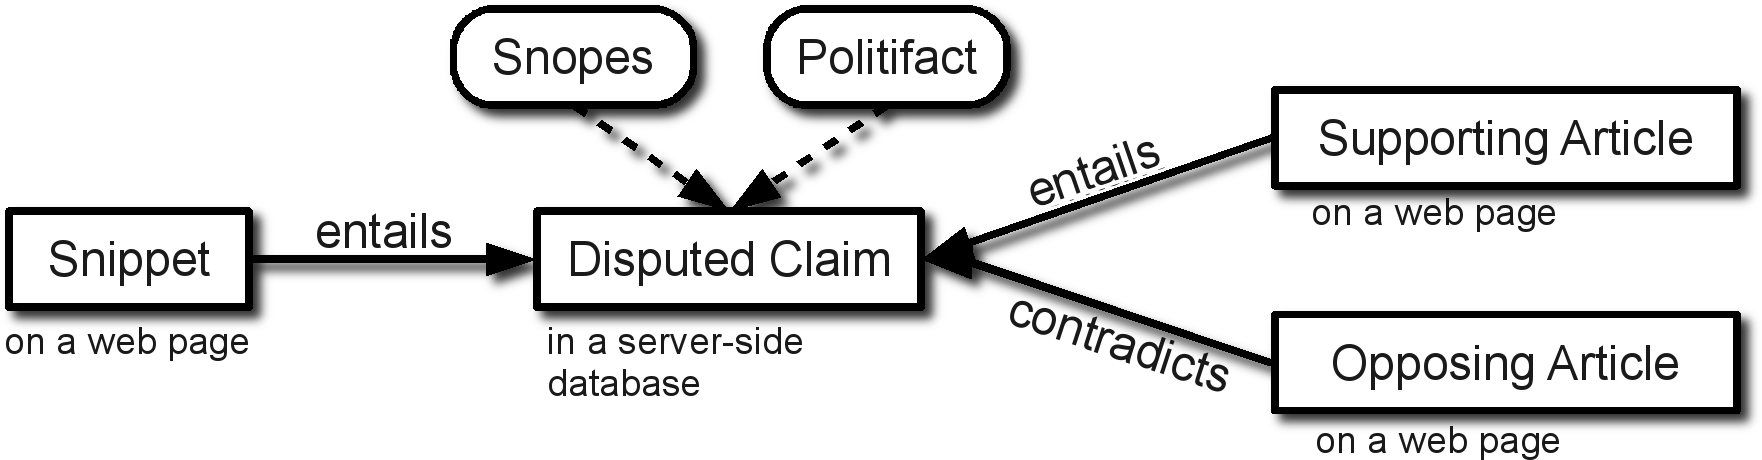
\includegraphics[width=8.5cm]{pictures/snippet_claim_article_fancy3.png}
	\caption{Snippets entail claims. Claims are entailed or contradicted by articles.}
	\label{snippet_claim_article}
	\end{center}
\end{figure}


\subsection{Personas}

If users are going to adopt Dispute Finder, it is important that it solves a real need. We used interviews to construct two personas which model the two ways that we expect a user to use Dispute Finder.

{\it Skeptical Readers} want to know when something they read is disputed by a source that they might trust. They are skeptical about the accuracy of the information that they read and often check multiple sources to get different opinions on a topic. A user will typically behave like a skeptical reader for some topics and not others. For example a user may be skeptical when reading about topics that affect them (e.g. health, things important to their job, or things they are expected to be knowledgeable about), but disengaged when reading about topics that do not affect them (e.g. entertainment).

{\it Activists} care strongly about particular issues and are prepared to spend some time informing others that something that they disagree with is disputed. They are the same kinds of people who join protest groups, write blogs, email news stories, or argue about topics online. They are motivated by a desire to influence others and to gain status by being seen to do so. A user is likely to be an activist on some issues, but not on others. An activist will often also be a skeptical reader.

Many users fall into neither of these two personas. If a user does not regularly read information online that they feel they need to need to understand well, or restricts their reading to sources that they believe they can trust, then they are unlikely to be interested in a tool like Dispute Finder.


\section{Background and Related Work}

There is ample evidence that at least some people are skeptical about the information they read and would like to know about alternative points of view that are supported by sources that they trust. This has lead to a growing set of tools that aim to help users deal with disputed and biased information.

According to Pew Research~\cite{PewResearch2008}, a substantial proportion of people regularly get information from sources that they do not fully trust. Their 2008 survey found that 33\% of Democrats regularly watch Fox News, and yet only 19\% believe all or most of what Fox News says. Similarly, 51\% of Democrats regularly watch CNN, and yet only 35\% believe all or most of what CNN says. While these figures are for TV News, rather than the web, Pew report that 48\% of web users people regularly follow search links to unfamiliar sources, and that users view online sources such as blogs with more skepticism that their print, broadcast, and cable counterparts. 

These findings were backed up by our interviews (Section~\ref{sec:interviews}). Several participants told us that they regularly get information from sources that they do not entirely trust. A user might read information from an untrusted source because the source is interesting, entertaining, linked to from somewhere else, or it came up in a search. For example they might read Michael Moore because he is entertaining, while having low opinions of his credibility, or they might read articles mailed to them by friends. 

\todo{Talk about people reading from a wide range of sources.}

There is also evidence that a significant group of people are interested in checking information they read on the web. Several popular web sites are designed primarily to help users check information they read elsewhere. For example Snopes.com contains information about urban myths such as ``eskimos have many words for snow'' and Factcheck.org and Politifact.com investigate claims made by American political figures. According to Quantcast.com, Snopes has around five million unique visitors per month.

To check these assumptions, we circulated a survey among members of a local debate club, who we anticipated would be a good match for our Skeptical Reader and Activist personals. Of the 23 people who responded, 91\% said that they sometimes or often check information they read on a trusted site (64\% often, 27\% sometimes) and 91\% said that they sometimes or often check information by searching for other web pages about the same topic (74\% often, 17\% sometimes).

\todo{Talk about our survey}

Fact checking web sites and search engines work well when you know something is disputed, but are of little use if you did not realize that what you were reading was disputed. The primary aim of Dispute Finder is to let you know when something you are reading is disputed.

Many other tools highlight disputed information on web pages. ReframeIt.com, ShiftSpace.org and SpinSpotter.com allow a user to manually annotate a web site that they disagree with, overlaying their own opinions on top of existing content. Videolyzer~\cite{Diakopoulos2008} allows users to comment on disputed claims in video clips. There are many other web annotation tools, including Google SideWiki, Annotea~\cite{Koivunen2001} and ScreenCrayons~\cite{Olsen2004}, each of which presents a different combination of features, and most of which could be used to annotate disputed content.

There are two key differences between Dispute Finder and these annotation tools: First, rather than allowing a user to express their own opinions about a topic, Dispute Finder instead requires a user who wants to promote a particular opinion to do so by linking to an article from a trusted source that argues for that opinion. Our interviews (Section~\ref{sec:interviews}) lead us to believe that most users would rather know that a trusted source disagrees with what is being written than that an unknown user disagrees.

The second key difference between prior annotation tools and Dispute Finder is that prior annotation tools allow a user to annotate {\it text on a particular page} while Dispute Finder attempts to allow a user to annotate a {\it general claim, everywhere it appears on the web, however it is worded}. If a user of an annotation tool adds an annotation to a page then their annotation will only appear on that page. If a user of Dispute Finder tells Dispute Finder to highlight a disputed claim, that claim will be highlighted on every web page on which Dispute Finder's algorithms determine that the claim appears. The closest annotation system to Dispute Finder in this respect is perhaps SparTag.us~\cite{Hong2009}, which uses an SHA hash to attach an annotation to an exact paragraph, irrespective of where it appears on the web; however a claim may be written in many different ways, and be part of many different paragraphs.

Several Sensemaking, Decision Support, and Argumentation tools allow a user to annotate a document with structured information that they may then share with other users. TRELLIS~\cite{Gil2002} helps a user annotate the rationale for their decisions and opinions by annotating source documents with the facts that they extracted from them, and connecting these facts into a decision graph. ClaimSpotter~\cite{Sereno2005,Sereno2004} applies a similar approach to scholarly papers, allowing a user to make up a paper with logical subject-verb-object triples describing important claims made in the document. Entity Workspace~\cite{Bier2006} uses entity extraction algorithms to allow an intelligence analyst to easily mark up a source document with facts extracted from it. Cohere~\cite{Shum2008} is a web based argumentation tool that allows people to connect {\it ideas} together using arbitrary verbs such as ``is an example of'', ``supports'', or ``challenges''. An idea can contain a link to a web page that contains that idea, and the Cohere Firefox Extension informs a user when the page that they are is the source for a known idea.

These tools allow a user to mark up the facts made by a single document, but do not provide facilities for a user to mark up large numbers of documents as being the same claim, or to automatically inform a user when other sources disagree with what they are reading.

There are also several tools that find pages write about the same topic with different slants, rather than looking at the specific claims a page makes. News Cube~\cite{Park2009} automatically finds articles that present different {\it aspects} of the same news story. The intention is that by reading several such aspects, the user will encounter several different ways of looking at the issue at hand, and will gained a broader perspective of the issue. 
Services such as Skewz.com and Newstrust.net allow users to rate news articles for bias. Skewz rates stories as being either liberal or conservative and encourages readers to read what the other side is thinking. Newstrust allows users to rate news articles for quality and objectivity. 

On Wikipedia, WikiTrust~\cite{Adler2008a} highlights passages on Wikipedia that are statistically likely to be reverted, based on how recently they were written and the track-record of the author, Wiki Dashboard~\cite{Kittur2008} creates a visualization of the edit history of a Wikipedia article that lets a user see how contentious it is, and Wiki Scanner\footnote{http://wikiscanner.virgil.gr} finds cases where a Wikipedia edit has been made by someone with a conflict of interest. These tools have a similar aim to Dispute Finder, but are limited to Wikipedia.

More generally, Dispute Finder is an example of an Open Hypermedia system~\cite{Bouvin2000,Wiil1996}. Like other Open Hypermedia systems, Dispute Finder lays an additional link structure over an existing hypertext document. In the case of Dispute Finder, the links are from disputed claims to information about those claims.

Dispute Finder also has some similarity to tagging tools~\cite{Marlow2006,Golder2006}. Tagging tools allow users to collectively categorize information by associating it with a user-created set of tags. In the case of Dispute Finder, the tags are disputed claims, and the tagged entities are sentences that make those claims. 


\todo{Improve the paraphraser UI so it shows users what pages are making the claim}
\todo{Improve the ``see examples on the web'' UI to it shows the pages that were found with the activists training work}
\todo{Provide a customized RSS reader and search engine that does dispute tracking. - future work?}
\todo{Should we explicitly list what we think are our key contributions?}


\section{Design}

Creating a tool to manage disputed information requires designers to address a number of challenges, including:

\begin{description}
\item[Developing a corpus of disputed claims:] To be useful, the set of known disputed claims needs to be both large and credible. If the database's coverage is too small then users will rarely see snippets highlighted. If the database is not credible then users will often see snippets highlighted for which there is no credible evidence for other points of view.

\item[Detecting these disputed claims on the web:] Given a particular web page, how do we determine which phrases on that page are making known disputed claims and should be highlighted? There is a trade-off between precision and recall. We do not want to highlight a snippet that is not making a disputed claim, but we do want to maximize the likelihood that we highlight a snippet that is making a disputed claim.

\item[Highlighting disputed claims for users:] If we are to alert a user when they read disputed information, we need to be able to tell what text they are reading, and we need a way to inform them that this information is disputed. Ideally, this method should apply to as much of the information the user reads as possible, and be easy for a user to adopt. We also want to avoid distracting the user unnecessarily, while also making sure that they notice disputed claims that they would care about.

\item[Providing tools that help users interpret disputed claims:] Once a user has learned that a claim is disputed, it is likely that they will want to see information that will help them decide whether they should believe the claim and what other sources they should read. We want to help a user understand both {\it who} holds other points of view and {\it why} other people hold different points of view.

\item[Determining Trustworthy Sources:] What sources should we consider ``trustworthy'' in the sense that their opinions are worth presenting to the user, and things that they disagree with should be highlighted as disputed. There is a trade-off between showing a user sources that they will trust, and showing them sources that will expose them to a new point of view.
\end{description}

These challenges are not unique to dispute finder; indeed they apply to any tool that informs a user about disputed information and helps users interpret this disputed information.

In the rest of this section, we discuss the various alternative solutions that we explored for each of these problems, and our experiences with the approaches that we implemented and tested.


\subsection{Developing a Corpus}
\label{sec:disputed}

Dispute Finder maintains a shared server-side database of known disputed claims. The browser extension highlights a text snippet if it believes that the snippet entails one of the claims in this database (Figure~\ref{snippet_claim_article}). Claims can either be added directly by users (Figure~\ref{add_claim}) or mined from web sites such as Snopes and Politifact that already maintain well curated databases of disputed claims, 

This database should not contain contain everything that has ever been disputed by anyone. In some sense almost everything is disputed by someone on the web. There are enough people writing enough opinions that if we alerted users every time anything they read was disputed by anyone then Dispute Finder would be so distracting as to be worthless. Similarly, there is little point spending effort rebutting claims that nobody believes. For example there is reliable evidence opposing the claim that the moon is made of cheese, but few people believe this claim is true. What we want is a set of claims that are widely believed and for which there is credible evidence supporting other points of view.

\begin{figure}[tb]
	\begin{center}
	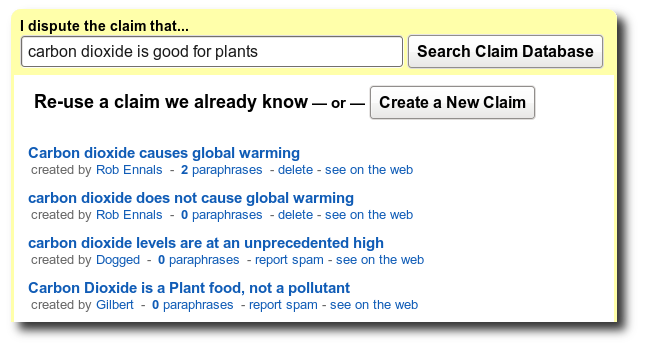
\includegraphics[width=8cm]{pictures/add_claim_list.png}
	\caption{A user can use this interface to add a new disputed claim manually.}
	\label{add_claim}
	\end{center}
\end{figure}

Currently most of our claims are automatically mined from Snopes and Politifact. Both of these sites maintain well curated databases of disputed claims, together with information about them. Snopes has good coverage of urban myths, and Politifact has good coverage of claims made by American politicians. In the future we plan to crawl other sites that cover other kinds of disputed claims (e.g. medical claims) and to provide an API to allow any site to provide a well-structured feed that we can use. At the time of writing, Dispute Finder has imported 1,457 claims from Snopes and 595 claims from Politifact.

One weakness of the automatic import approach is that the claims found on these sites are often phrased differently to the way they commonly appear on the web. For example many of the claims on Politifact are exact quotes such as ``One-third of the health care dollar goes to no such thing as health care; it goes to the insurance companies''. In practice, it is often necessary for users to enter several simple paraphrases for a claim before it can be reliably detected.

Dispute Finder also provides users means to add their own disputed claims using the Dispute Finder web interface (Figure~\ref{add_claim}). The web interface is modeled after common issue-reporting software such as Uservoice.com and Bugzilla.org. It first encourages the user to search the existing database to see if their claim already exists, and then allows them to create a new claim. When the claim is first added it is marked with a warning, informing the user that the claim will not be highlighted for other users until they have added at least one opposing article. At the time of writing, users have added 557 claims, and 140 users have added at least one claim.

%The automatic import bootstraps Dispute Finder with a useful database of disputed claims without needing a large active user community, and the crowd-sourcing aspect allows users to clean up claims that were not phrased well when imported, and add claims that are not part of any of our input feeds.

An alternative approach would be to use Contradiction Detection~\cite{Ritter} to find frequently repeated statements that appear to contradict statements from trusted sources. Unfortunately at the time of writing, Contradiction Detection does not seem to be robust enough for us to use it for this purpose.

In future work, we hope to automatically find disputed claims on the web by looking for phrases like ``falsely claimed that X'' --- a similar techniques to that used by Hearst to find hyponyms~\cite{Hearst1992}, and then use context to help determine which phrases are likely to be making the same claim.

\todo{Say how many disputed claims}
\todo{talk about duplicates}
\todo{Actually import the Politifact data}


\subsection{Detecting Known Disputed Claims}

Dispute Finder highlights a snippet if it thinks it entails the truth of a known disputed claim. This is complicated by the fact that a claim can be phrased in many different ways, and a snippet does not need to explicitly state a claim in order to entail its truth. For example ``I prefer margarine to butter because it is healthier'' entails ``margarine is healthier than butter''. Our implementation maintains a local copy of our claim database inside the browser extension and runs a simple textual entailment algorithm inside the browser to look for sentences that appear to entail known disputed claims. 

There is a trade-off between precision and recall. We want to maximize the likelihood that Dispute Finder will highlight a snippet if it is making a known disputed claim, while minimizing the likelihood that it will highlight a snippet that is not making a known disputed claim. We implemented and tested four different approaches that represent different points along this trade-off:

\begin{figure}[tb]
	\begin{center}
	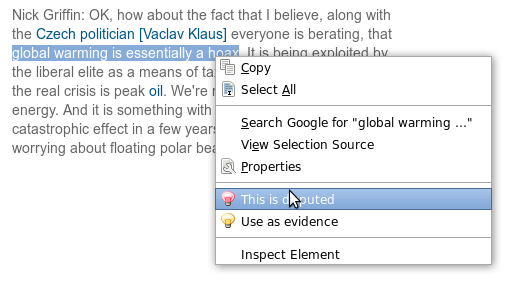
\includegraphics[width=6cm]{pictures/mark_disputed.png}
	\caption{Explicit page marking: select the snippet and click ``this is disputed'' on the context menu.}
	\label{mark_disputed}
	\end{center}
\end{figure}

\begin{figure}[tb]
	\begin{center}
	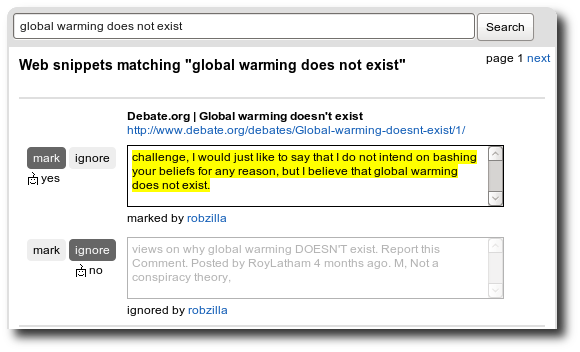
\includegraphics[width=7cm]{pictures/training2.png}
	\caption{Bulk page marking and server-side classification: classifier guesses are shown below the choice buttons.}
	\label{training}
	\end{center}
\end{figure}

\begin{figure}[t]
	\begin{center}
	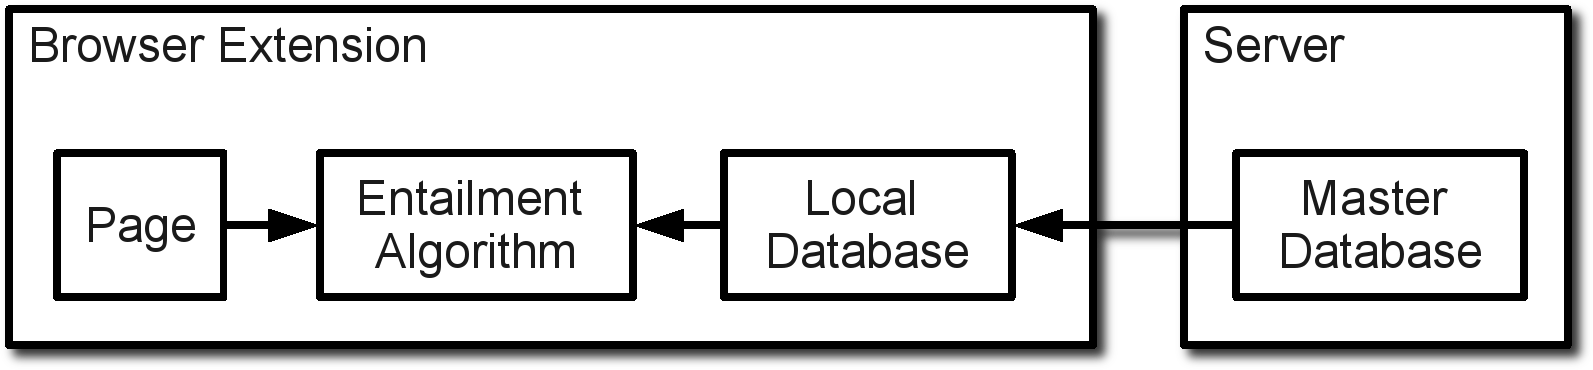
\includegraphics[width=8cm]{pictures/nlp_client_server2.png}
	\caption{Client-side entailment: the entailment algorithm runs on the client, using a claim database downloaded from the server.}
	\label{nlp_client_server}
	\end{center}
\end{figure}

\begin{figure}[tb]
	\begin{center}
	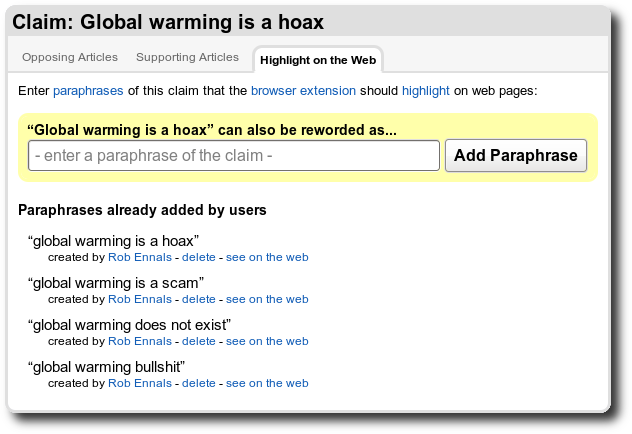
\includegraphics[width=8cm]{pictures/paraphrases.png}
	\caption{Users can enter paraphrases of a claim to help the entailment algorithm.}
	\label{paraphrases}
	\end{center}
\end{figure}


\label{sec:explicit_mark}
\begin{description}
\item[Explicit page marking:] The user explicitly marks a snippet on a page by selecting the snippet, and selecting ``mark as disputed'' from a context menu (Figure~\ref{mark_disputed}).

\item[Bulk page marking:] The user uses a search interface to rapidly gather many snippets that contain similar phrases, and then selects those that they would like to mark (Figure~\ref{training}). The server uses Yahoo BOSS\footnote{http://developer.yahoo.com/search/boss} to search the web for snippets that resemble a paraphrase entered by the user. 

\item[Server-side classification:] The server uses the examples from the bulk page marking interface to train a classifier. We used a simple Bayesian classifier with n-grams as features. The classifier looks at the positive and negative examples given by the user and learns n-grams that should or should not be present in a snippet in order for it to make the claim.  Once the classifier has been trained, the server uses it to refine which other results from Yahoo BOSS should be marked (Figure~\ref{training}).

%We have only partially implemented this approach.
\todo{Should we say that we didn't completely finish this version?}

\todo{Has anyone done something like this before.}
\todo{We only partially implemented this approach}

\item[Client-side entailment:] The browser extension runs a simple textual entailment algorithm over all sentences on every web page the user browses, checking to see if any sentence on the page entails any claim in the database (Figure~\ref{nlp_client_server}). A user can enter additional paraphrases of a claim to help the entailment algorithm (Figure~\ref{paraphrases}). This is the implementation used by the released version of Dispute Finder.
\end{description}

Explicit page marking has the highest precision, but the poorest coverage. Since a user is looking at the page in its entirety, they can read the snippet in context and make a good judgment about whether the snippet is indeed making the claim. However the manual effort required per page makes it difficult for this approach to scale. We also found that it can also be hard to motivate a user to mark snippets if they think that it is unlikely that another user with the Dispute Finder extension will read exactly this page. This same problem has hindered the adoption of numerous web page annotation tools.

Bulk page marking trades off some precision for better coverage. When a user searches for a phrase, they can quickly find hundreds of snippets and mark them by clicking on them. Since they are reading the snippet out of context, they are more likely to mark a phrase incorrectly. 

Server side classification trades off more precision for more coverage. The classifier can mark more pages than a user could ever mark manually, and can keep marking new pages as they appear, but it is inevitably less accurate than a human.

Client side entailment gets the most coverage. Since the classification algorithm is run inside the client, the client can highlight snippets on pages that the server has not examined. This is particularly important for news pages, which are frequently read only a few minutes after they are posted. Moreover, the client-side approach can highlight snippets on web pages that would not be accessible to the server, such as web-based email, and intranet sites. 

A further advantage of the client-side approach is that it avoids the need for the client to give the server any information about what pages the user is browsing. The list of all URLs and snippets that make disputed claims is too large and updates too frequently for it to be practical for the client to store it locally, so the client instead asks the server for information about each URL the user browses, reducing user privacy. By contrast, the list of paraphrases is small enough and changes slowly enough that the client can maintain its own local copy of the database, removing the need for the client to tell the server what pages the user is browsing. As our database grows bigger, it will of course become more challenging to maintain a local copy in the browser extension.

\subsubsection{Textual Entailment}

Detecting entailment between texts is a semantic analysis problem. Our client side entailment method uses the standard Local Lexical Matching (LLM) algorithm~\cite{Jijkoun2006} that is a common baseline to which other algorithms are often compared~\cite{Braz}. Our implementation divides the page into sentences, strips out stop-words, does stemming, and then looks for sentences that contain the keywords contained in a paraphrase of a known claim. If the claim contains a negation word (e.g. not, never, can't) then so must the matching sentence. To improve performance, rather than always running the LLM algorithm on every sentence on every page the user browses, the client starts by quickly scanning the page for ``hot terms'' such as ``Global Warming'' that are known to appear in disputed claims. The hot terms are selected such that every claim contains at least one hot term. If a hot term is found, then the sentence that contained the hot term compared against all claims about that hot term.

LLM is far from being state of the art and many more sophisticated textual entailment algorithms exist. Modern approaches include treating the sentence as a logical formula and attempting a logical proof~\cite{Bayer2001,Bos2005}, parsing each phrase into a syntax tree and using syntax heuristics~\cite{Snow2006}, inferring inference rules that can transform one sentence into another while preserving meaning~\cite{Lin2001,Dinu2009,Bhagat2009}, and using Bayesian inference to infer whether one phrase looks like the kind of phrase that would have included each word in the other phrase~\cite{Glickman2005}. Tools such as AuContraire~\cite{Ritter} focus specifically on detecting contradictions. Several tools rely on an underlying information extraction tool such as TextRunner~\cite{Etzioni2008}.

While Dispute Finder would almost certainly improve its precision and recall if it used a more sophisticated algorithm, LLM has the advantage of being simple enough to run efficiently inside a user's web browser for every page they look at without causing a noticeable slowdown. We do however believe that there is scope to use more sophisticated algorithms, particularly as processor speeds improve.


\todo{Mention that we could add the +ve and -ve n-grams to the client code? Actually do this?}

\todo{Discuss how and why this is simpler than the server-side classification method}
\todo{Explain how we avoid downloading the entire database}

\todo{Should we have a version where the interface merely suggests n-grams that should be used by the classifier}
\todo{Can we present all these systems without giving detailed stats about how they compare?}
\todo{Add support for a user to enter 'anti-phrases' when a snippet is wrongly highlighted}
\todo{Add support for a user to enter a paraphrase that will match the snippet they are looking at}
\todo{Do a load more people in a final user-study round. Try to get it up to 8.}
\todo{Explain how our algorithm relates to existing NLP work - due to unusual domain}


Other authors have used similar algorithms to find repeated information on the web. Kolak and Schilit~\cite{Kolak2008} look for passages places where one book quotes another, qSign~\cite{Kim2009} looks for places where one blog has quoted another, and duplicate-detection is often used to clean up web searches~\cite{Theobald2008}. MemeTracker~\cite{Backstrom2009} looks for phrases shared by multiple news stories, accounting for minor variations, and uses this to track the way that news flows between traditional news sources and blogs.

The authors of MemeTracker observed that many ideas often flow around the web in the form of ``memes'' that are repeated on many web sites with relatively little variation. To the extent that this is true, it simplifies identifying snippets that repeat the idea. MemeTracker uses this to track the way an idea propagates across the web using a relatively simple algorithm. We have found that the precision and recall of our client-side textual entailment algorithm varies hugely depending on how meme-like a claim is. Some claims (particularly those derived from quotes) are widely repeated almost-verbatim, and can be detected relatively easily. However many other claims are rarely stated explicitly in a single sentence or with the same choice of words, making them much harder to detect with a simple algorithm.

\todo{Give an example of a good meme}

\todo{Talk about what dispute finder does, and how it differs - maybe by moving this into the main system section}
\todo{Cite plagarism detection}
\todo{Talk about how our algorithm looks for key terms used in disputed claims}
\todo{Talk about how our first pass NLP algo is rather like }


\subsection{Highlighting Disputed Claims}

\begin{figure}[tb]
	\begin{center}
	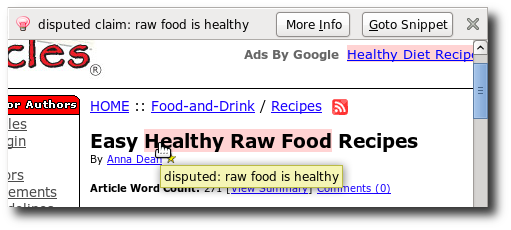
\includegraphics[width=8cm]{pictures/highlight_bar.png}
	\caption{Dispute Finder highlights text snippets that make disputed claims, and displays a notification bar to inform the user that they should look out for highlighted snippets.}
	\label{highlight_bar}
	\end{center}
\end{figure}

%Dispute Finder is designed to alert a user when information they read on a web page makes a claim that is disputed by a source they might trust. 
%
%
%Dispute Finder aims to inform users when information they read on the web makes claims that are disputed by sources that they might trust. We are particularly interested in informing users about claims that they hadn't thought about before, hadn't realized were disputed by sources they repect, or have not yet established a strong opinion on.

The Dispute Finder Firefox extension uses two mechanisms to inform a user when information on the page they are reading is disputed. It highlights any disputed snippets in red, and it displays a notification bar (Figure~\ref{highlight_bar}). 

The notification bar alerts the user that they should look out for highlighted snippets. Highlights can be difficult to see if the page is using a background that is similar to our highlight color\footnote{We tried to choose a color that is easily distinguished from most background commonly used background colors.} particularly if the user is color blind. The notification bar also allows a user to step through the highlighted snippets on the page.

The highlights show a user {\it which snippets} Dispute Finder believes are making disputed claims. A user can see whether the highlights are in the text that they are reading and ignore disputed snippets in text that they are not interested in - such as user comments. The highlights also allow a user to see when Dispute Finder has incorrectly inferred that a phrase as making a disputed claims that it is not making. In such cases, the user is encouraged to help Dispute Finder improve its marking by clicking on the disputed claim and clicking on the ``report incorrect highlighting'' button from the popup interface.

Once a user is aware that a claim is disputed, there is little point telling them about the same disputed claim again in the future. We have not yet concluded whether it is better for Dispute Finder to automatically stop highlighting a claim once a user has viewed the claim, or whether it is better for a user to explicitly ask Dispute Finder to stop highlighting a claim. In our current implementation, a user can tell Dispute Finder to not highlight a claim again by setting the ``don't highlight this claim for me again'' checkbox in the popup interface (Figure~\ref{claimview}). Requiring a user to manually opt out of a claim requires more work from the user, but hiding already viewed claims can be confusing, since users do not normally expect viewing something to be a destructive operation. A compromise position is to highlight claims that have been seen before in a fainter color; similar to the way links are typically colored on web pages.

\todo{Try using a fainter color}

\todo{Text is wrong in the screenshot}

Dispute Finder also provides an API that allows other sites to determine whether their content makes disputed claims. For example, a search engine could inform a user if its results contained disputed claims, or an RSS feed reader could tell a user if a news story makes disputed claims.

\todo{Document API online}
\todo{Change the highlight color to yellow? Auto-adjust highlight color based on background color?}
\todo{Should we automatically adjust the highlight color, based on the background color of the page}
\todo{Discuss previous work on highlighting here, rather than in related work?}



\subsection{Helping Users Interpret Claims}

When a user clicks on a highlighted snippet, Dispute Finder displays a popup pane with information intended to help the user determine whether there are alternative points of view that they should take seriously, and whether there are articles on this topic that they should read. In our current implementation, the popup interface shows lists of articles that support or oppose the claim (Figure~\ref{article_list}). We also implemented and tested an interface that contained a user-editable argumentation graph; however we found that users had difficulty creating such graphs and were more interested in {\it who} disagreed with a claim than {\it why} people disagreed with it.

We could have omitted this claim-information feature and still had a useful system. Once a user sees that something is disputed, they could use an alternative service, such as a search engine, Wikipedia, Politifact or Snopes, to find further information about the claim. There are however several reasons why it makes sense for Dispute Finder to maintain information about a disputed claim:

\begin{description}
\item[Convenience:] A user may not have the patience to search for a good source of information about a claim. 
\item[Moderation:] We only want Dispute Finder to highlight a claim if we know that there is credible evidence for an alternative point of view. By storing the evidence for alternative points of view inside Dispute Finder, it becomes easier for a moderator user to evaluate whether a claim is sufficiently disputed that it belongs in the Dispute Finder database.
\item[Filtering:] Although we have not implemented this feature currently, we think it could be useful to build a model of what sources a user trusts and only highlight a disputed claim if a source that the user trusts argues against it.
\end{description}


We prototyped and tested two different ways of showing a user alternative points of view to the disputed claim they are looking at:

\begin{figure}[tb]
	\begin{center}
	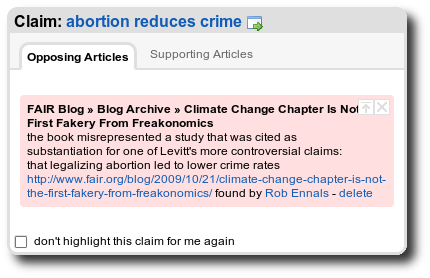
\includegraphics[width=6cm]{pictures/popup_abortion_shadow.png}
	\caption{Article List interface for a disputed claim}
	\label{article_list}
	\end{center}
\end{figure}



\begin{description}
\item[Argumentation graph:] When the user clicks on a snippet that makes a disputed claim, Dispute Finder shows them a simple user-editable argumentation graph. This graph is inspired by IBIS~\footnote{Issue Based Information System} tools such as gIBIS~\cite{Conklin1987a}, Compendium~\cite{Selvin2001}, Zeno~\cite{Gordon1997}, and Cohere~\cite{Shum2008}. Each claim is linked to claims that represent alternative points of view, and claims that support that point of view. Each claim also has a list of articles that argue in favor of that claim (Figure\ref{popup_graph})

\item[Article lists:] Dispute Finder shows the user two lists of articles, one of which contains articles arguing in favor of the claim, and the other of which contains articles arguing against the claim (Figure~\ref{article_list}). For each article, the interface shows a summary sentence that captures the core argument used by the article. A user can add any web page as a supporting article by browsing to the page, selecting ``use as evidence'' from a context menu (Figure~\ref{add_article}) and then saying what claim it supports or opposes (Figure~\ref{article_choose}).
\end{description}

The argumentation graph makes it easier to see {\it why} a claim is disputed, while the article lists make it easier to see {\it who} supports or opposes the claim. 

\begin{figure}[tb]
	\begin{center}
	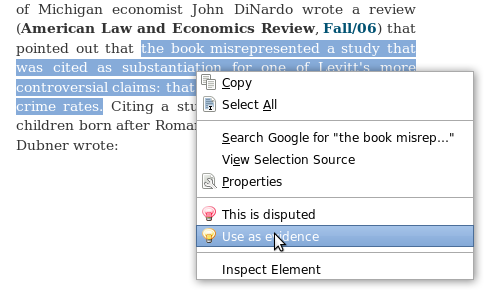
\includegraphics[width=6cm]{pictures/mark_evidence.png}
	\caption{To add an article, select some summary text, and click ``use as evidence'' from the context menu.}
	\label{add_article}
	\end{center}
\end{figure}

\begin{figure}[tb]
	\begin{center}
	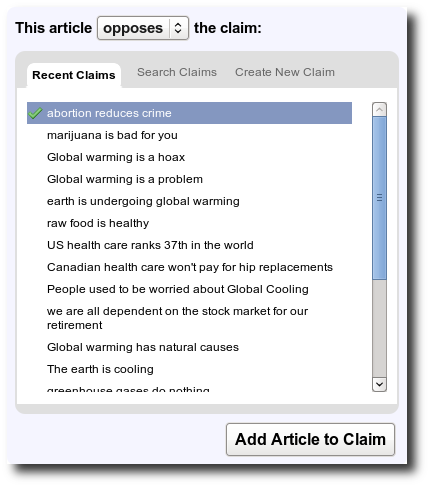
\includegraphics[width=6cm]{pictures/article_choose_claim.png}
	\caption{Choose how to connect an article with a claim.}
	\label{article_choose}
	\end{center}
\end{figure}

\todo{Call them supporting pages? Naming is a mess right now.}

When using the article list approach, several different articles may be making essentially the same argument and it may not be obvious that one of the articles is making a point that the user had not come across before. The argumentation graph allows the user to easily see what the range of different opinions is, and quickly see if there is an argument that they have not encountered before. 

A significant weakness of the argumentation graph approach is that a good argumentation graph takes significantly more effort to build than a simple list of articles. In our prototype the argumentation graph was built entirely by users and we found that our users had difficulty creating graphs that were useful for other users. There were two problems here: first, breaking down all the different arguments for and against a claim takes much more time than just adding articles to a list, particularly given that a single article will often make several different opposing points; second, we found that users had difficulty creating well structured argumentation graphs, as we outline in Section~\ref{user-studies}. This result is consistent with previous studies~\cite{Isenmann1997}.

Another point in favor of using a simple list of sources is that most of the users we talked to seemed to be more interested in {\it who} disputed a claim, rather than what their argument was. For example, if a user is a reader of the New York Times, and they hear that the New York Times argues against the claim they are reading, then they will take the dispute much more seriously than if the key article arguing against the claim is from a source they are not familiar with. Moreover, we found that when a user wanted to understand {\it why} a claim is disputed, they preferred to read whichever article seemed to be most credible, rather than browsing an argumentation graph.

It is possible that the best solution would be a visualization that made it easy for a user to see both {\it who} was supporting/opposing a particular claim, and what arguments were being put forward.


\subsection{Determining Trustworthy Sources}

When showing articles to a user, it is important that these be from sources that the user would be likely to trust. In the current version of Dispute Finder, a user can add any web page as a source, but users are requested to restrict themselves to pages that meet the Wikipedia criteria\footnote{http://en.wikipedia.org/wiki/Wikipedia:SOURCES} for being reliable. Good sources of articles include newspapers, universities, respected organizations, and Wikipedia itself. A user can vote on whether they think a particular article is useful, and this voting determines the order in which articles are listed. A user can also request that an article be deleted they believe the source does not meet credibility requirements, or if it is not relevant to the claim. These requests are forwarded to moderator users who have the power to delete links to articles.

Unfortunately, as Pew Research discovered~\cite{PewResearch2008} when looking at TV news, while most people say they want to receive information ``without a point of view'', the sites people actually trust are often those that share the person's own point of view. It seems that ``without a point of view'' is a similar concept to ``without an accent''. Similarly, Manjou~\cite{Manjou2008} reports that people tend to measure the credibility of a source based on how well it fits with what they already believe to be true.  As a consequence, there may be little point showing liberal sources to a conservative, or vice-versa. Similarly, a global voting system can be gamed by people who vote up weak arguments against claims they support in order to hide stronger arguments. Moreover, by using moderators to decide which sources and claims are high enough quality to be presented to other users, we open ourselves up to charges of bias.

It may thus be better to learn what sources a particular user is likely to believe are reliable, and then adjust both what sources Dispute Finder shows to the user, and what claims are highlighted, based on this.

There is a difficult trade-off here. If we only show users sources that we believe they are likely to trust and only highlight claims as disputed if they are disputed by sources that share the user's own world-view then we risk reinforcing the echo-chamber effect that Dispute Finder is intended to fight against. On the other hand, if we only provide information from sources that are widely regarded as being reliable, we risk enforcing the beliefs of the establishment and stifling the voices of those who are less accepted by the establishment but may still be right. If we pay no attention to what sources the user trusts, or what sources are generally regarded as credible, then we may waste time trying to persuade users using sources that they would not take seriously. We do not yet claim to know a good solution for this problem, but we believe it is an interesting area for further research.

\todo{Cite Pew Research study saying people like to read news that supports their own point of view, but many others like neutral sources. http://people-press.org/report/?pageid=1353}

Other researchers have looked at ways to determine what sources a user will trust. 
BJ Fogg et al~\cite{Fogg2003} found that the most important factor was whether a web site had a professional-looking design. Gill and Arts~\cite{Gil2006} identified on a different set of factors, including topic (a medical site may not be trusted for advice on car repair), popularity (does everyone else use this) and authority.


\section{Evaluation}
\label{sec:interviews}
\label{user-studies}

We gathered information from users using user-studies and a set of interviews. We performed three qualitative ``think aloud'' user studies and interviewed most of our user study participants, along with six additional people. The aim of these studies was to inform the iterative design of the Dispute Finder tool. The studies were not intended to validate the design of Dispute Finder as being correct. 

We found that most people were interested in having a tool like Dispute Finder, and were able to use Dispute Finder effectively as a Skeptical Reader. However we found that users were frustrated by the relatively low fraction of disputed claims that Dispute Finder currently highlights, and had some difficulty adding new claims themselves.


\subsection{Procedure}

For the first two studies, we recruited participants using Craigslist. We posted a message asking people to tell us how they used the web to form and promote their opinions and used their responses to select people who we thought might fit our ``skeptical reader'' and ``activist'' personas. For the final study, we instead used people from our lab who we thought would be a good fit for our personas. The first study had twelve participants (five female, seven male), the second study had six participants (four female, two male), and the final study had six participants participants (all male). 

Each batch of users was shown a different iteration of the Dispute Finder design. The first two batches used versions in which users marked snippets explicitly and in which the popup window explaining a claim showed an argumentation graph describing the structure of the different alternative points of view (Figure~\ref{popup_graph}). The final group used a version in which a textual entailment algorithm on the client was used to determine what to mark, and the popup window showed lists of articles that support or oppose the claim. We present the findings of the three user studies together. Where a comment refers to particular version we make this clear.

\begin{figure}[tb]
	\begin{center}
	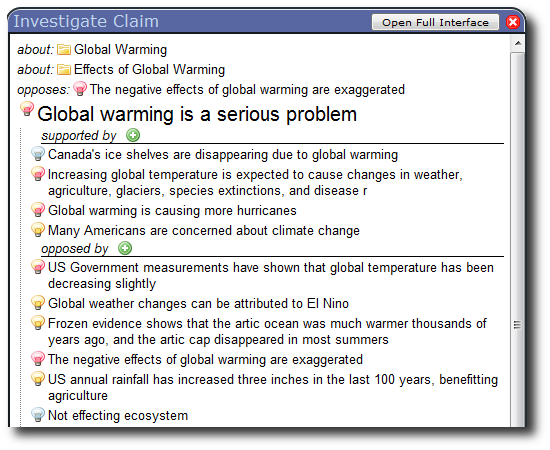
\includegraphics[width=8cm]{pictures/popup_graph_crop.png}
	\caption{Argumentation graph interface for a disputed claim}
	\label{popup_graph}
	\end{center}
\end{figure}


Study sessions took approximately forty five minutes. Participants were seated at a workstation with the Firefox browser augmented with the Dispute Finder extension. They were asked to view pages that had highlighted claims on them, and to attempt to add new disputed claims to our database.

We also conducted interviews with most of our user study participants, and five additional people, asking them how they use the web to form and promote their opinions.

\todo{Need to finish the third wave of user studies}

\subsection{Findings}

Responses were generally positive. Most of the participants expressed an interest in using the tool ``when it is more mature'' with some keen to use it in its current state.

\todo{Tye: say how many were keen to use the tool.}

Most participants said that they would want to use Dispute Finder to tell them when information they read was disputed (skeptical reader). One participant said ``The web needs to be taken with a grain of salt, and this gives you salt goggles''. A smaller number said they would be likely to enter claims they disagreed with (activist). One participant who was a political blogger was eager to mark things he thought were lies.

Most users were able to use Dispute Finder competently as a skeptical reader (browsing information about disputed claims) but found it harder to act competently as an activist (adding new disputed claims). Several participants wanted to see Dispute Finder work for them as a skeptical reader before dedicating time to adding and curating new claims (``I want to see it work before I add stuff'').

When browsing a page that had disputed claims highlighted, most users correctly inferred that these were sentences they should be skeptical about, but some users thought Dispute Finder was saying the sentences were wrong, rather than merely disputed. Not all users realized that one could click on a highlighted snippet to bring up more information. Several users complained about Dispute Finder highlighting snippets that were not making the claim Dispute Finder indicated.

Most users were frustrated by the relatively poor precision and recall that Dispute Finder has at present. Several users browsed to a page that they knew contained disputed claims, and were disappointed when Dispute Finder did not highlight anything. Several users were also frustrated when Dispute Finder highlighted phrases that did not make the claim Dispute Finder indicated. If Dispute Finder is to be adopted widely then we will need to significantly improve precision and recall, by building a bigger database of disputed claims, and improving the accuracy of our textual entailment algorithm.

Most people we interviewed were interested in applying Dispute Finder to particular areas that affected them (e.g. health) or that they were expected to be knowledgeable about (e.g. something relating to their work), but were less interested in applying it to pages about topics that they were less interested in. For topics that did not affect them users felt that misinformation was ``not important enough to bother with'', or that they could ``afford to be misinformed''. Users said they read about some topics (e.g. celebrity gossip) ``for entertainment'' or ``to relax'' and so they were less interested in making sure they properly understood those topics.

%In the first study, a user could mark a snippet by 
%
%In the interface used in the first two studies, a user could mark a snippet by selecting it, right clicking on it, and clicking ``mark as disputed''. They were then prompted to either select an existing claim or create a new one.

\subsubsection{Claims}

When using explicit page marking (Section~\ref{sec:explicit_mark}) to mark a snippet on a particular page, many users often did not appreciate that a claim should apply to more than one snippet. Several users tried to create a new claim with exactly the same text as the snippet they were marking, and several users asked why they had to ``enter the text again''. Similarly, several users got confused when a snippet made two different disputed claims. The correct behavior is to mark the same text with two different claims, but several participants tried to create a new compound claim such as ``Global warming will cause X and Y''. 

Conversely, when adding a claim to the Dispute Finder web site, users would often enter claims that are not disputed anywhere on the web or enter paraphrases that do not resemble the wording used on any web site. The challenge of how to help users come up with claims that occur on many web sites is one that we have not yet solved.

Several users expressed confusion about how specific a claim they created should be. For example, if a snippet says ``Global temperatures will rise by X degrees by 2050'' then is that making the claim ``Global temperatures will rise'', or should the claim include the extra information? In order to make a good judgment, one needs to know the range of similar claims that are being made by other web sites, and what claims there is good evidence against. If one makes the claim too specific then one will be able to find less web pages that make it, but if one makes the claim too general then it might be harder to find solid evidence against it.

Several users got confused by claims that referred to similar events at different points in time. For example, one participant in the first study marked one claim as opposing another claim when they were referring to similar incidents that occurred at different times. 

Several users created claims that had ambiguous meanings. One user entered a disputed claim about ``Wood'', meaning the guitarist ``Ronnie Wood'' of the Rolling Stones. Similar problems occurred with claims that were specific to a particular country, or a particular point in time. 


\subsubsection{The Article List}

When adding sources that support or oppose a claim, a user would frequently mark the first paragraph of the article rather than seeking out the sentence that best summarized the argument that the article was using against the claim. In some cases the first paragraph is indeed the right text to select, since the first paragraph is typically a summary of the core argument made by the articles; however there was often a better choice available. Several users wanted to mark up a table or image as the summary of an article, which is not currently supported.

When using the article list interface (Figure~\ref{article_list}), several users got confused about whether an article supported or opposed a claim that was phrased negatively. For example a user would mark an article that opposed global warming as opposing the claim ``global warming is bad'' because the article opposed global warming.

Several users expressed an interest in being able to add a disputed claim without having to find opposing evidence. One user said that opposing a claim required ``too many clicks'' and they wanted to be able to just vote against a claim without having to say why or find evidence. Users did however recognize that they would want to see opposing evidence as a reader.

\subsubsection{The Argumentation Graph}

In the first two studies, the popup interface for a claim showed an argumentation graph (Figure~\ref{popup_graph}). This graph connected the claims in our database using ``supports'' or ``opposes'' links, and allowed each claim to also be associated with supporting articles. When shown an argumentation graph for a claim, users seemed to have little difficulty navigating and understanding it and appreciated the ability to explore the structure of an argument and see how different claims were connected. One user said ``I can see myself getting addicted to this'', and another said ``it's very intuitive''.

Users seemed to have difficulty creating such graph structures however. Several users linked one claim as supporting another when it would have been more logically correct for them to both support a third claim. For example ``Global warming is causing more hurricanes'' does not support ``Global warming is causing rising sea levels'', but both support ``Global warming is causing problems''. Users correctly realized that the claims were related, but were not sure how best to connect them. Some users were confused by claims that had a ``because'' relationship rather than a ``supports'' or ``opposes'' relationship. For example ``America did not sign the Kyoto Protocol'' {\it because} ``Signing Kyoto would harm the US economy''. These findings are consistent with those of Isenmann and Reuter~\cite{Isenmann1997}.




\todo{Need to say that the argumentation graph contains all existing claims and that it was a simple ``supports"/``opposes'' graph.}

\todo{Come up with terminology for marking an evidence snippet, and agree on evidence vs source vs article}
\todo{Talk about how the early versions conflated evidence and snippets - and whether it makes sense to distinguish between them}
\todo{Screenshot of the claim graph interface}


\section{Conclusions and Future Work}

We have introduced the idea of Dispute Finder, an Open Hypermedia tool that informs a user when a web page they are reading is making a claim that is disputed by a source they might trust. We have discussed the key challenges that one must address in order to make a system like this work, proposed several solutions to these challenges, and discussed our experiences with those solutions that we have implemented and tested with users.

As we discuss in this paper, our system requires multiple components to work in concert. Performing the tasks associated with these components well is a hard problem, and we do not yet claim to have an implementation that is is good enough to be compelling for most users. We do however believe that Dispute Finder attacks an interesting problem that, if solved well, could significantly improve the utility of the web.

At the time of writing 11,729 people have installed and tried out Dispute Finder, 2,297 are active daily users, 140 have added new claims to our database, 149 have added articles, and our database contains 2,609 disputed claims. 

An experimental preview version of Dispute Finder is available at 
\url{http://disputefinder.org}


\todo{Add count of disputed claims}

%\section{Acknowledgments}

\todo{Do we want to have acknowledgements}
% We would like to Thank Barbara Rosario for help with textual entailment, and 
% Acknowledgements omitted for blind submission. Dispute Finder uses icons from the free FamFamFam Silk\footnote{http://famfamfam.com} collection.


\todo{Sort out bad references}
\bibliography{refs}

\end{document}



